\documentclass{article}

% if you need to pass options to natbib, use, e.g.:
%     \PassOptionsToPackage{numbers, compress}{natbib}
% before loading neurips_2021

% ready for submission
\usepackage[preprint]{neurips_2023}

% to compile a preprint version, e.g., for submission to arXiv, add add the
% [preprint] option:
%     \usepackage[preprint]{neurips_2021}

% to compile a camera-ready version, add the [final] option, e.g.:
%     \usepackage[final]{neurips_2021}

% to avoid loading the natbib package, add option nonatbib:
%    \usepackage[nonatbib]{neurips_2021}

\usepackage[utf8]{inputenc} % allow utf-8 input
\usepackage[T1]{fontenc}    % use 8-bit T1 fonts
\usepackage[colorlinks=true]{hyperref}       % hyperlinks
\usepackage{url}            % simple URL typesetting
\usepackage{booktabs}       % professional-quality tables
\usepackage{amsfonts}       % blackboard math symbols
\usepackage{nicefrac}       % compact symbols for 1/2, etc.
\usepackage{microtype}      % microtypography
\usepackage{xcolor}         % colors
\usepackage{graphicx}
\usepackage{cleveref}

\title{Corporate vs. Academia: Who Dominates CV Conferences?}

% The \author macro works with any number of authors. There are two commands
% used to separate the names and addresses of multiple authors: \And and \AND.
%
% Using \And between authors leaves it to LaTeX to determine where to break the
% lines. Using \AND forces a line break at that point. So, if LaTeX puts 3 of 4
% authors names on the first line, and the last on the second line, try using
% \AND instead of \And before the third author name.

\author{%
  Irem Karaca\\
  Matrikelnummer 6939373\\
  \texttt{@student.uni-tuebingen.de} \\
  \And
  Merve Kocabas\\
  Matrikelnummer 7040890\\
  \texttt{merve.kocabas@student.uni-tuebingen.de} \\
  \And
  Hari Joshithaa Aghilah Senthilprathiban\\
  Matrikelnummer 6943473\\
  \texttt{hari-joshitha.aghilah-senthilprathiban@student.uni-tuebingen.de} \\
  \And
  Shubham Raheja\\
  Matrikelnummer 7001572\\
  \texttt{@student.uni-tuebingen.de} \\
}

\begin{document}

\maketitle

\begin{abstract}
  % \emph{[Use this abstract to briefly explain what you are planning to do. Here is an example:]} We are planning to use the collection of \href{https://openreview-py.readthedocs.io/en/latest/getting_data.html}{all papers ever \emph{submitted} to the ICLR conference} to see how well paper acceptance can be predicted from trivial features, such as the paper's overall length, number of words or number of figures. We are planning to use logistic regression for this purpose.

  In this project, we analyse the corporate and academia involvement in popular Computer Vision conferences such as CVPR, ICCV and WACV. 
\end{abstract}

% You can find a detailed example and instructions on how to use this style file in the attached \texttt{neurips\_2023.tex} file. This includes instructions for how to lay out citations.

\section{Introduction}


\section{Data and Methods}
DATASET (dataset parts, collection, reprocessing, facts about dataset etc.)

Methods (spearman rank correlation, one-tailed t-test)


\section{Results}
To explore the hypothesis—Do papers from corporate-affiliated researchers have more influence at top-tier computer vision conferences?—we begin by examining the trend in the quantity of corporate-affiliated papers over the years. As shown in Figure \ref{fig:corporate_ratio_graph}, the proportion of corporate-affiliated papers has steadily increased across major computer vision conferences. CVPR, ICCV, WACV, and the combined dataset all exhibit a consistent upward trend, with corporate involvement reaching its highest levels in recent years. However, despite this increase, academia continues to dominate these conferences, as the highest ratio of corporate-affiliated papers remains at 0.47. Additionally, while ICCV and CVPR show relatively higher levels of corporate affiliation, WACV consistently lags behind them in this regard. The Spearman rank correlation results in Table \ref{tab:spearman_results} further support the observation in consistent upward trend in corporate affiliation, with strong positive correlations (coefficients exceeding 0.88) and statistically significant p-values (all below 0.05). These findings illustrate the growing presence of corporate-affiliated research within the academic ecosystem of top-tier computer vision venues.

\begin{figure}[ht]
  \centering
  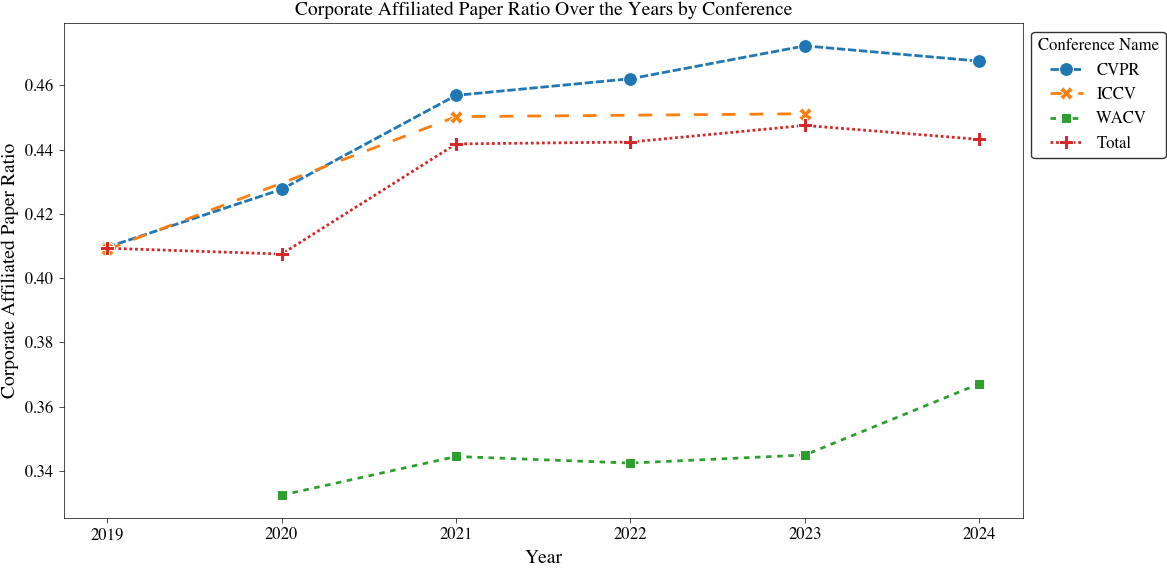
\includegraphics[width=\textwidth]{report/images/corporate_ratio_graph_final.png}  
  \caption{Corporate affiliated paper ratio over the years for each conference and total dataset.}
  \label{fig:corporate_ratio_graph}
\end{figure}

\begin{table}[ht]
\centering
\begin{tabular}{|l|c|c|c|}
\hline
\textbf{Conference} & \textbf{Spearman Rank Correlation} & \textbf{P-value} & \textbf{Significant Relationship?} \\ \hline
CVPR & 0.9429 & 0.0048 & Yes \\ \hline
ICCV & 1.0000 & 0.0000 & Yes \\ \hline
WACV & 0.9000 & 0.0374 & Yes \\ \hline
Total & 0.8857 & 0.0188 & Yes \\ \hline
\end{tabular}
\caption{Spearman rank correlation results for each conference and total dataset.}
\label{tab:spearman_results}
\end{table}

Building on the observed upward trend in the number of corporate-affiliated papers, we now turn our attention to their impact. A critical metric for evaluating research influence is citation count, which reflects the reach and recognition of a paper within the scientific community. To assess this, we compare the citation performance of corporate-affiliated papers to those from academia across top-tier computer vision conferences. Specifically, we examine whether corporate-affiliated papers, despite their lower overall proportion, exhibit higher citation counts, thereby offering insight into their relative impact as hypothesized. 

In order to evaluate the IEEE citation counts, we first analyse the distributions of corporate and academia affiliated paper citations. As illustrated in \cref{fig:ieee_citations}, the number of academia papers seem to be more for lower citation counts and academia papers seem to be more prevalent for higher citation counts.  

\begin{figure}
    \centering
    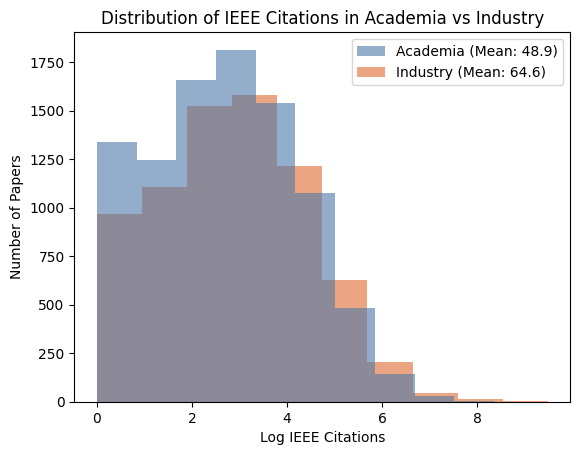
\includegraphics[width=0.6\linewidth]{images/histogram_ieee_citations.png}
    \caption{Distribution of IEEE Citations for Academia and Industry Papers}
    \label{fig:ieee_citations}
\end{figure}

To test if industry affiliated papers have a higher mean citation count ($\mu_2$) than the mean citation of academic papers ($\mu_1$), we perform a one sided T-Test. We set $\alpha$ to be 0.05. The null $(H_0)$ and alternative hypothesis $H_\alpha$ are stated below as follows,

\[
H_0 = \mu_2 \leq \mu_1 (\mathrm{Industry \  IEEE \  citations \ have\  a \ smaller\  or\  equal\  mean \ than\  Academic\  papers})
\]

\[
H_\alpha = \mu_2 \geq \mu_1 (\mathrm{Industry \ IEEE\ citations \ have \ a \ higher\ mean \ than \ Academia \ papers)}
\]

The test results in a p-value of $1.05 \times 10^{-7}$. Thus, we can reject $H_0$, and say that there is a statistically significant difference to indicate that the Industry papers have a higher IEEE citation mean than Academia affiliated papers. 

After observing the upward trend in the number of corporate-affiliated papers and their higher IEEE citation counts, it becomes essential to further explore which types of corporations are driving this influence in top-tier computer vision conferences. The dominance of large corporations is particularly striking as shown in Figure \ref{fig:corporate_size_graph}. Big companies contribute over 60\% of corporate representation and nearly 80\% of affiliated papers, solidifying their central role in shaping the research landscape. This is not surprising given that computer vision research often requires immense computational resources, including high-performance hardware, access to large-scale datasets, and advanced machine learning infrastructure—factors that demand significant financial investment. Such resources are more readily available to large corporations, enabling them to produce impactful research and maintain a strong presence in these conferences. The list of the top 10 companies with the highest number of papers—Google, Facebook, Microsoft, Huawei, Adobe, Tencent, Alibaba, Amazon, Nvidia, and Apple—further supports this trend, as all are classified as big companies. This imbalance highlights the challenges faced by smaller organizations, such as scaleups and startups, which often lack the resources to compete at the same level. This concentration of research output raises important questions about the extent to which corporate priorities shape the direction of computer vision research. To address the corporate priorities, we analyzed the key research areas explored by corporate and academic-affiliated papers at these top-tier computer vision conferences. 

\begin{figure}[ht]
  \centering
  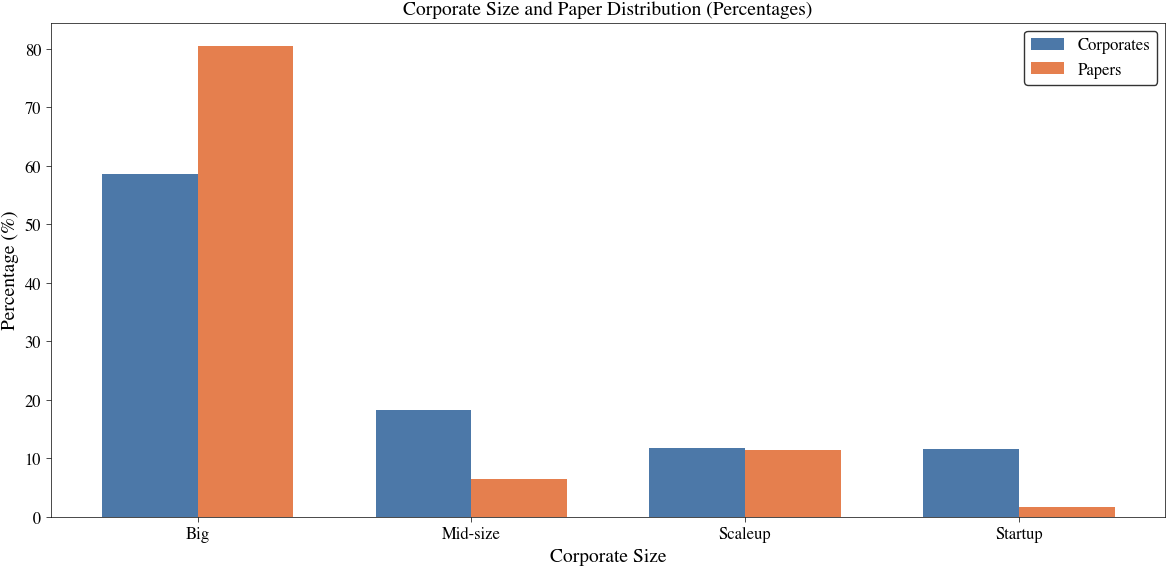
\includegraphics[width=\textwidth]{report/images/corporate_paper_distribution.png}  
  \caption{Corporate size and paper distribution in percentages.}
  \label{fig:corporate_size_graph}
\end{figure}

RESEARCH FOCUS AREAS

\section{Discussion and Conclusion}

\section{Future Work}

\section{Contributions Statement}
% This is the last section before the references. 

% \emph{Here is an example:}

% XX performed the correlation analysis, organized the data and code for the processing of dataset1 and subdataset2, and created the scatter plot. 
% YY created the random forest regression model, performed the data cleaning for the xyz analysis / xyz database, and created the bar charts to display the regression results. 
% ZZ researched and collected the raw data, restructured the pipeline for the data analysis, and proof-read the draft for the final report. 
% AA performed the data cleaning for dataset1, and performed the Ridge and Lasso regularization. 
% All members of the group contributed to writing the report.

\section*{References}

\end{document}
